\documentclass{article}
\usepackage{leonine,amsmath,amssymb,amsthm,graphicx}
\setkeys{Gin}{width=\linewidth,totalheight=\textheight,keepaspectratio}
\graphicspath{{graphics/}}
% Prints a trailing space in a smart way.
\usepackage{xspace}
% Inserts a blank page
\newcommand{\blankpage}{\newpage\hbox{}\thispagestyle{empty}\newpage}
% \usepackage{units}
% Typesets the font size, leading, and measure in the form of 10/12x26 pc.
\newcommand{\measure}[3]{#1/#2$\times$\unit[#3]{pc}}

\theoremstyle{definition}
\newtheorem{pred}[thm]{Prediction}

\title{Cerebellum: Mathematical Preliminaries} \author{Eric Purdy}

\begin{document}

\maketitle

\section{Probability Space}

A finite probability space\footnote{It is slightly more complicated to
  define an infinite probability space, so we will assume that our
  probability spaces are finite.} is a finite set $\Omega$ together
with a function $P$ from $\Omega$ to the real numbers $\RR$, such that
\begin{itemize}
\item For all $\omega \in \Omega$, $0 \le P[\omega] \le 1$
\item $\sum_{\omega\in \Omega} P[\omega] = 1$
\end{itemize}

The elements $\omega$ of $\Omega$ are called {\em elementary events}.
An {\em event} is a subset $S$ of $\Omega$, and its probability is the
sum of the probabilities of the elementary events that make it up:
$$P[A] = \sum_{\omega \in A} P[\omega].$$ We say that the event $A$
happens if we pick a sample $\omega$ from $\Omega$ and $\omega \in A$,
and that it does not happen if $\omega \notin A$.

For us, $\Omega$ will generally be the space of all possible
activities of neurons in the brain at a single instant in time. One of
the most common events that we will be interested in is the event that
a particular neuron $s$ fires; there are many possible states of the
brain that include $s$ firing (for example, every single neuron in the
brain firing, or $s$ alone firing and no other neuron in the brain
firing), and these are the elementary events that make up the event
``$s$ fires''.

\section{Random Variables}

A random variable is a function $X$ from a finite probability space
$\Omega$ to some set. For our purposes, the set will always be $\RR$,
the real numbers.

For a random variable $X$, and a real number $a \in \RR$, the event
that $X=a$ is just the subset of those $\omega$ in $\Omega$ such that
$X(\omega) = a$. The probability of this event is written as $P[X=a]$.
If we write just $P[X]$, this should be understood as a function that
maps values of $X$ to probabilities, i.e., $P[X](a) = P[X = a]$.

If $X$ and $Y$ are random variables, then so are $aX$, $X+Y$, $X-Y$,
$X\cdot Y$, and $\frac{X}{Y}$. These are the functions 
\begin{align*}
(aX)(\omega) &= a \cdot X(\omega)\\
(X+Y)(\omega) &= X(\omega) + Y(\omega)\\
(X-Y)(\omega) &= X(\omega) - Y(\omega)\\
(X\cdot Y)(\omega) &= X(\omega) \cdot Y(\omega)\\
\left(\frac{X}{Y}\right)(\omega) &= \frac{X(\omega)}{Y(\omega)},\\
\end{align*}
respectively. In this way, we can build up more complicated random
variables from simpler ones.

The {\em expected value} or {\em average value} of a random variable
$X$ is defined to be
$$E[X] = \sum_{\omega \in \Omega} P[\omega] X(\omega).$$

\section{Conditional Probabilities}

We will be working with conditional probabilities. The {\em
  conditional probability of A given B}, written $P(A|B)$, is the
probability that event $A$ happens given that we already know that $B$
has happened. It is defined as the probability that both $A$ and $B$
happen (written $A\cap B$) divided by the probability that $B$
happens.
$$P[A|B] = \frac{P[A \cap B]}{P[B]}$$

Two events $A$ and $B$ are said to be independent if $P[A|B] = P[A]$.

If $X$ and $Y$ are random variables, then the events we are interested
in are the event that they take on a particular value. A conditional
probability $P[X|Y]$, where $X$ and $Y$ are random variables, should
be understood as a function that maps values of $X$ and $Y$ to
probabilities, i.e., $P[X|Y](\alpha, \beta) = P[X=\alpha | Y=\beta]$.

It is always the case that, for every $\beta$, $\sum_\alpha
P[X=\alpha|Y=\beta] = 1$, where the sum is taken over all possible
values of $A$.

Two random variables $X$ and $Y$ are said to be independent if the
events $X=a$ and $Y=b$ are independent for every $a$ and $b$.

\section{Covariance}

The {\em covariance} between two random variables is defined as 
$$Cov[X,Y] = E[XY] - E[X]E[Y].$$
The covariance is higher if $X$ and $Y$ tend to be large at the same
time and small at the same time. If it is zero, $X$ and $Y$ are said
to be ``uncorrelated''. Two independent random variables are always
uncorrelated, but two uncorrelated random variables need not be
independent.

\section{Partial Derivatives}

\begin{figure}
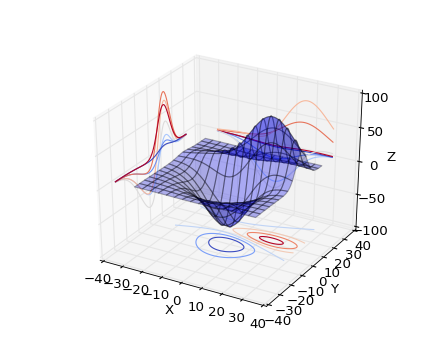
\includegraphics[width=\linewidth]{contour3d_demo3.png}
\caption{A function of two variables. The partial derivative is the
  derivative of the curves shown on the left and right walls.}
\label{fig-partial}
\end{figure}

The partial derivative of a function $f(x_1, \dots, x_n)$, denoted by
$\frac{\partial f(x_1, \dots, x_n)}{\partial x_i}$, is the derivative of
the function
$$g(x) = f(a_1, \dots, a_{i-1}, x, a_{i+1}, \dots, a_n),$$
where the $a_j$ are constants. Some functions $g$ are shown for
different values of the $a_j$ in Figure \ref{fig-partial}, for a
function of two variables $f(x_1, x_2)$.

\section{Stochastic Gradient Ascent/Descent}

Let $f$ be a function of $n$ real variables $x_1, \dots, x_n$. We want
to find the values of $x_1, \dots, x_n$ for which $f(x_1, \dots, x_n)$
is largest. For completely general $f$, this is impossible to do
except by a brute force search over the entire space, which is
impossible, since there are infinitely many settings for each
$x_i$. For functions $f$ which are continuous and which have
continuous derivatives, it is still nontrivial, and often the best we
can do is to find a setting of the $x_i$ which is locally highest,
i.e., such that there is no $x_1', \dots, x_n'$ close to $x_1, \dots,
x_n$ such that $f(x_1', \dots, x_n') > f(x_1, \dots, x_n)$.

We can find local maxima of continously differentiable $f$ by
repeatedly taking small steps in the direction that makes the function
grow fastest:
$$\Delta x_i = \eta \cdot \frac{\partial f(x_1, \dots, x_n)}{\partial
  x_i}.$$ 
The notation $\Delta x_i$ means that we replace $x_i$ by $x_i + \Delta
x_i$.  Here $\frac{\partial f}{\partial x_i}$ is a partial derivative;
it specifies how fast $f$ will grow if we take a small step in the
direction of increasing $x_i$. This procedure is called {\em gradient
  ascent}; if we are trying to minimize a function, we simply go in
the opposite direction:
$$\Delta x_i = -\eta \cdot \frac{\partial f(x_1, \dots, x_n)}{\partial
  x_i}.$$ This is called {\em gradient descent}.

The parameter $\eta$, called the ``learning rate'', controls how fast
we move in the direction of the gradient. Lower rates result in more
accurate gradient computations (since we are updating our direction
more frequently), but also result in gradient ascent taking
longer. Learning rates that are too high can result in oscillation
around the desired solution, as the algorithm keeps overshooting the
best point. Learning rates are generally set empirically, by seeing
what works best in a particular context.

It is often easier to find a random variable whose average value is
the gradient, and use that instead of the true gradient in our
updates. This is called {\em stochastic} gradient ascent or descent,
depending on whether we are trying to maximize $f$ or minimize $f$.
More formally, if we have random variables $Y_i$ ($i=1, \dots, n$)
such that:
$$\frac{\partial f(x_1, \dots, x_n)}{\partial x_i} = E[Y_i] = \sum_a P[Y_i=a]
a,$$ and we have a source of random samples $y_i(1), \dots, y_i(T)$
of $Y_i$, then we can maximize $f$ via the update
$$\Delta x_i = \eta \cdot y_i(t).$$ 

In general, the partial derivative of $f$ will change as the $x_i$
change, so we will need a new random variable $Y_i$ at each time
step. Fortunately, this is often possible. In general the approach
taken is to use a single sample from each random variable, then update
the $x_i$ according to the update rule above, then pick a new random
variable whose expected value is the new gradient.

It is important to note that there may be many different random
variables whose expectation is equal to the gradient. For instance, if
we have a random variable such that $E[X]$ is equal to a gradient of
interest, then the same is true of the random variable
$$X + a\frac{I[X \ge 0]}{P[X \ge 0]} - a \frac{I[X<0]}{P[X < 0]},$$
where $I[X \ge 0]$ is one if $X \ge 0$ and zero otherwise, and
$I[X<0]$ is one if $X<0$ and zero otherwise. We therefore do not
require that the neurological evidence exactly match the stochastic
gradient descent equations we give.

One random variable that seems especially biologically plausible is
$$T_{X, a} = E[X | X\ge a] I[X \ge a] + E[X | X < a] I[X < a],$$
where
$$E[X | X \ge a] = \sum_{\omega: X(\omega) \ge a}X(\omega)
\frac{P[\omega]}{P[X \ge a]},$$ 
and similarly for $E[X | X < a]$. The random variable $T_{X,a}$ has
the same expectation as $X$, but has the very simple form of a step
function: it has one constant value when $X<a$ and another constant
value when $X\ge a$.
\end{document}
